% This is samplepaper.tex, a sample chapter demonstrating the
% LLNCS macro package for Springer Computer Science proceedings;
% Version 2.20 of 2017/10/04
%
\documentclass[runningheads]{llncs}
%
\usepackage{graphicx}
\graphicspath{ {./images/} }
\usepackage[utf8]{inputenc}
\usepackage[spanish,es-nodecimaldot]{babel}
\usepackage[spanish, fixlanguage]{babelbib}
% Used for displaying a sample figure. If possible, figure files should
% be included in EPS format.
%
% If you use the hyperref package, please uncomment the following line
% to display URLs in blue roman font according to Springer's eBook style:
% \renewcommand\UrlFont{\color{blue}\rmfamily}

\begin{document}
%
\title{Consejo de embajadores: una variación del Naming Game basado en comunidades}
%
%\titlerunning{Abbreviated paper title}
% If the paper title is too long for the running head, you can set
% an abbreviated paper title here
%
\author{Diego de Jesús Isla López \and
Saul Ivan Rivas Vega}
%
% First names are abbreviated in the running head.
% If there are more than two authors, 'et al.' is used.
%
\institute{Universidad Nacional Autónoma de México, Ciudad Universitaria, Ciudad de México, México\\
\email{\{abc,saul.ivan.rivas.vega\}@comunidad.unam.mx}}
%
\maketitle              % typeset the header of the contribution
%
\begin{abstract}
El Naming Game es una simulación basada en agentes los cuales con un protocolo de comunicación y una memoria buscan llegar a un acuerdo sobre que única palabra almacenar para nombrar a un objeto. En el presente trabajo extendemos las características del diseño original propuesto por Baronchelli, con el propósito de reportar y analizar las diferencias en los parámetros de estudio durante la simulación. Se llevaron a cabo una serie de experimentos por cada combinación posible dentro de un espacio reducido de valores y la media de resultados son los tomados en cuenta para el análisis. Los resultados mostraron que... De igual forma presentamos nuestras conclusiones y trabajo a futuro. 

\keywords{Naming Game  \and Comunicación \and Agentes \and Inteligencia Artificial \and Simulación.}
\end{abstract}
%
%
%
\section {Introducción}
Se han realizado trabajos con experimentos basados en la hipótesis de que el lenguaje es un sistema adaptativo que se forma así mismo a través de un proceso cultural auto-organizado~\cite{ref_article1}.

Ahora revisemos la definición de los juegos del lenguaje que fueron propuestos por primera vez en las investigaciones filosóficas de Ludwig Wittgenstein en 1967~\cite{ref_article1}. Su modelo consiste en considerar a un constructor y a un asistente con distintas herramientas y recursos los cuales el constructor debía solicitar al asistente, lo cual llevaba a comunicarse en un lenguaje primitivo. Sin embargo Wittgenstein no creía que así era como se comportaba el lenguaje en el mundo real. Lo que el pensaba era que podían reconocerse particularidades de la lingüística que si se asemejan al mundo real.

Posteriormente se realizaron implementaciones de variada complejidad como lo son: \textit{Naming Games}~\cite{ref_article1}, \textit{Guessing Games}~\cite{ref_article1}, \textit{Descripting Games}~\cite{ref_article1}, etc.
\section{Antecedentes}
El trabajo propuesto en Naming Games~\cite{ref_article1} inspiró el trabajo de Baronchelli~\cite{ref_article1} para desarrollar un modelo de comunicación entre agentes. En dicho modelo se utilizaba el siguiente protocolo de comunicación entre el hablante y el escucha que son 2 agentes seleccionados al azar:
\begin{itemize}
	\item El hablante selecciona un objeto del contexto actual
	\item El hablante toma una palabra de su inventario para referirse al objeto, en caso de no tener una palabra, crea una nueva.
	\item El hablante comunica la palabra seleccionada al receptor
	\item Si el escucha tiene en su inventario la palabra que le comunicó el hablante, la comunicación se considera exitosa lo que hace que tanto el hablante como el escucha borren su inventario de palabras para el objeto con excepción de la palabra que ambos conocen.
	\item En caso contrario el escucha almacena en su inventario de palabras la palabra que le comunicó el hablante.
\end{itemize}
\section{Diseño Propuesto}
\subsection{Protocolos de comunicación}
\subsection{Generación de palabras}
\subsection{Evaluación de preferencia}
\subsection{Convergencia}
\section{Experimentos}
Descripción de las distintas combinaciones.
\section{Resultados}
\section{Discusión y Conclusiones}
\section{Introducción}
\subsection{A Subsection Sample}Please note that the first paragraph of a section or subsection is
not indented. The first paragraph that follows a table, figure,
equation etc. does not need an indent, either.

Subsequent paragraphs, however, are indented.

\subsubsection{Sample Heading (Third Level)} Only two levels of
headings should be numbered. Lower level headings remain unnumbered;
they are formatted as run-in headings.

\paragraph{Sample Heading (Fourth Level)}
The contribution should contain no more than four levels of
headings. Table~\ref{tab1} gives a summary of all heading levels.

\begin{table}
\caption{Table captions should be placed above the
tables.}\label{tab1}
\begin{tabular}{|l|l|l|}
\hline
Heading level &  Example & Font size and style\\
\hline
Title (centered) &  {\Large\bfseries Lecture Notes} & 14 point, bold\\
1st-level heading &  {\large\bfseries 1 Introduction} & 12 point, bold\\
2nd-level heading & {\bfseries 2.1 Printing Area} & 10 point, bold\\
3rd-level heading & {\bfseries Run-in Heading in Bold.} Text follows & 10 point, bold\\
4th-level heading & {\itshape Lowest Level Heading.} Text follows & 10 point, italic\\
\hline
\end{tabular}
\end{table}


\noindent Displayed equations are centered and set on a separate
line.
\begin{equation}
x + y = z
\end{equation}
Please try to avoid rasterized images for line-art diagrams and
schemas. Whenever possible, use vector graphics instead (see
Fig.~\ref{fig1}).

\begin{figure}
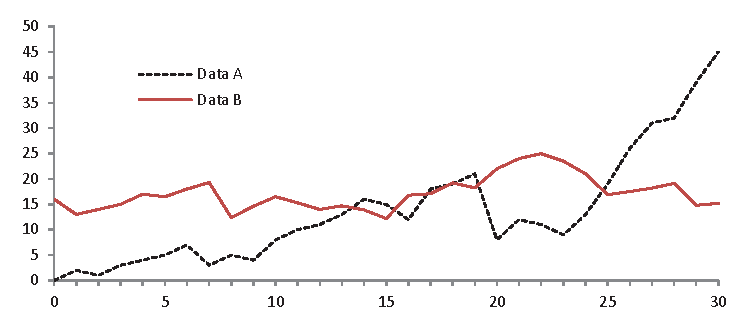
\includegraphics[width=\textwidth]{fig1.eps}
\caption{A figure caption is always placed below the illustration.
Please note that short captions are centered, while long ones are
justified by the macro package automatically.} \label{fig1}
\end{figure}

\begin{theorem}
This is a sample theorem. The run-in heading is set in bold, while
the following text appears in italics. Definitions, lemmas,
propositions, and corollaries are styled the same way.
\end{theorem}
%
% the environments 'definition', 'lemma', 'proposition', 'corollary',
% 'remark', and 'example' are defined in the LLNCS documentclass as well.
%
\begin{proof}
Proofs, examples, and remarks have the initial word in italics,
while the following text appears in normal font.
\end{proof}
For citations of references, we prefer the use of square brackets
and consecutive numbers. Citations using labels or the author/year
convention are also acceptable. The following bibliography provides
a sample reference list with entries for journal
articles~\cite{ref_article1}, an LNCS chapter~\cite{ref_lncs1}, a
book~\cite{ref_book1}, proceedings without editors~\cite{ref_proc1},
and a homepage~\cite{ref_url1}. Multiple citations are grouped
\cite{ref_article1,ref_lncs1,ref_book1},
\cite{ref_article1,ref_book1,ref_proc1,ref_url1}.
%
% ---- Bibliography ----
%
% BibTeX users should specify bibliography style 'splncs04'.
% References will then be sorted and formatted in the correct style.
%
% \bibliographystyle{splncs04}
% \bibliography{mybibliography}
%
\begin{thebibliography}{8}
\bibitem{ref_article1}
Author, F.: Article title. Journal \textbf{2}(5), 99--110 (2016)

\bibitem{ref_lncs1}
Author, F., Author, S.: Title of a proceedings paper. In: Editor,
F., Editor, S. (eds.) CONFERENCE 2016, LNCS, vol. 9999, pp. 1--13.
Springer, Heidelberg (2016). \doi{10.10007/1234567890}

\bibitem{ref_book1}
Author, F., Author, S., Author, T.: Book title. 2nd edn. Publisher,
Location (1999)

\bibitem{ref_proc1}
Author, A.-B.: Contribution title. In: 9th International Proceedings
on Proceedings, pp. 1--2. Publisher, Location (2010)

\bibitem{ref_url1}
LNCS Homepage, \url{http://www.springer.com/lncs}. Last accessed 4
Oct 2017
\end{thebibliography}
\end{document}
